\section{Method}\label{sec:method}

\Cref{fig:arch} shows the pipeline. Three principles guided every design decision.
\textbf{P1, calibrate, do not threshold:} every observation is scored against the incident's own history and peers, and
likelihoods use rates rather than cut-offs.
\textbf{P2, causes precede and propagate directionally:} errors travel up the call graph to callers and load travels down to
callees; a symptom the root can explain is not evidence against it, and load that came from upstream is not evidence for a
downstream root.
\textbf{P3, the LLM reads text and chooses among ranked options:} the decision and its evidence are computed.
The method has a core (stages 1--3 and the chain) and seven switchable modules: \Mod{1}--\Mod{6} form the statistical core
(\core{}), and \Mod{7} is the bounded LLM. All constants are listed in \cref{tab:constants} (\ref{app:constants}); none was fitted
to labels.

\begin{sidewaysfigure}
\centering
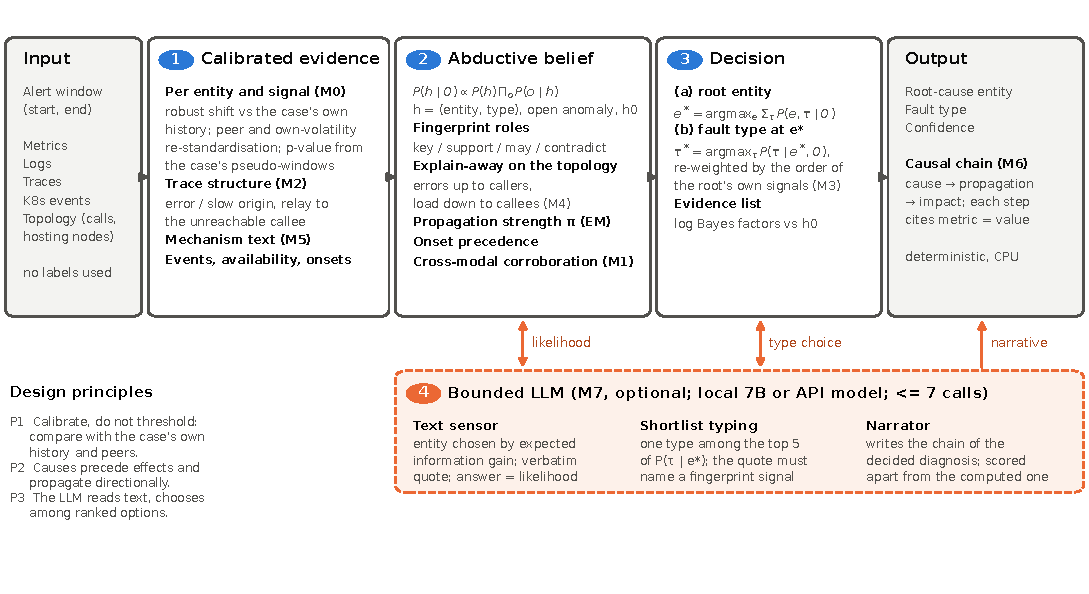
\includegraphics[width=\textheight]{figs/fig1_architecture.pdf}
\caption{\gama{}. Stage 1 turns telemetry into calibrated binary observations; stage 2 computes a posterior over (entity, fault
type) hypotheses; stage 3 decides the root entity and then its type; the chain (\Mod{6}) cites window values along the topology
path. The bounded LLM (stage 4, optional) contributes a likelihood term (sensor), a choice among the statistical shortlist (typing)
and a narrative that is scored separately.}\label{fig:arch}
\end{sidewaysfigure}

\subsection{Stage 1: calibrated evidence}\label{sec:evidence}

\paragraph{Signals}
Metric series are mapped to signal families by their names (CPU, memory, garbage collection, threads, disk, throttling, request
count, latency, errors, restarts, replicas / availability); configuration constants (limits, initial sizes) are excluded. For a
service the signals are, for instance, \sig{svc_cpu_rise}, \sig{svc_latency_rise} or \sig{svc_request_drop}; for a node
\sig{node_cpu_rise}, \sig{node_mem_rise}, \sig{node_disk_rise} and \sig{node_ready_drop}. Each signal has a direction
$d\in\{+1,-1\}$ (rise or drop).

\paragraph{Robust shift}
Let $x$ be a series of entity $e$ and $[a,b)$ a tested window of length $L=b-a$. Its history is $\mathcal{H}=[a-BL,a)$ with $B=4$.
The directional robust shift is
\begin{equation}\label{eq:shift}
\begin{aligned}
z &= d\cdot\frac{\median_{t\in[a,b)} x_t-\median_{t\in\mathcal{H}} x_t}{\sigma_{\mathcal{H}}},\\
\sigma_{\mathcal{H}} &= \max\!\big(1.4826\,\mad_{\mathcal{H}}(x),\;0.05\,|\median_{\mathcal{H}} x|,\;\epsilon\big),
\end{aligned}
\end{equation}
computed only when the history covers at least 80\% of its expected samples and the window at least half of them. Error counts are
summed in 30\,s bins (zero-filled) with a scale floor of one event per bin. The score of a signal is the largest $z$ over the
entity's series of that family.

\paragraph{Pseudo-windows and calibration}
A shift score is not a probability: series drift and are autocorrelated, so the window and its history are not exchangeable, and a
plain rank test flagged about 30\% of fault-free windows in our development runs. We therefore compute the same score on $K=5$
pseudo-windows $W_j=[w_0-jL,\,w_0-(j-1)L)$ cut from the incident's own pre-alert data, each against its own history. Two
re-standardisations are applied identically to real and pseudo scores. \emph{Own volatility}: each entity's score is re-centred and
re-scaled by the median and MAD of its pseudo scores (leave-one-out for the pseudo-windows, floor 1), so a chronically noisy entity
does not outrank one that changed only now. \emph{Peers}: in every window the score is re-standardised against the scores of the
other entities of the same kind (at least three peers, floor 1), which rejects a load step or a drift that moves all of them. The
calibrated p-value of the real window is the conformal rank of its score among the pseudo scores of all entities of the same kind
and signal in the incident \citep{efron2004null,vovk2005conformal},
\begin{equation}\label{eq:pvalue}
p = \frac{1+\#\{z'\in\mathcal{N}_{k,s}: z'\geq z\}}{|\mathcal{N}_{k,s}|+1},
\end{equation}
pooled over the entity kind when fewer than 20 pseudo scores exist. The signal \emph{holds} when $p\leq\alpha=0.05$. The
\emph{onset} of a holding signal is the first sample whose shift against a history ending one window earlier reaches 3 for two
consecutive samples.

\paragraph{Categorical observations}
Kubernetes events (OOM kill, crash loop, failed probe, scheduling failure, scale-down, restart, eviction, node not ready) count only
when their increments inside the window exceed their own long-run rate (Poisson test). Availability below the desired replica count
is a state. Failing spans contribute their HTTP / gRPC status class and the mechanism named by their message (null pointer, rate
limit, DNS, connection refused, timeout, Redis, out of memory, GC, thread pool, queue, load balancer, network policy, SQL, cache);
failing or slow dependency spans (database, cache, queue) are separate signals. The background rate of a categorical observation is
the share of entities of the same level showing it in the incident, shrunk towards $\alpha$ with a Beta prior worth ten
pseudo-entities. Each incident yields on the order of $10^3$ binary observations
$o=(e,s,\textit{holds},\textit{onset})$.

\subsection{Stage 2: abductive belief}\label{sec:belief}

\paragraph{Hypotheses}
For every service $e$ and fault type $\tau$ of service level, and every node and type of node level, $h=(e,\tau)$ is a hypothesis;
each entity also has an open hypothesis ``anomaly of unspecified type'', and $h_0$ denotes no fault. A hypothesis is \emph{testable}
only if at least one of its key signals was computed. The posterior is
\begin{equation}
\Pr(h\mid O)\;\propto\;\Pr(h)\prod_{o\in O}\Pr(o\mid h),
\end{equation}
with equal prior mass per entity, split among its hypotheses (the two fallback types of the taxonomy, \emph{httpError5xx} and
\emph{codeDefect}, at half weight), and $\Pr(h_0)=0.1$.

\paragraph{Fingerprint roles}
For each type, a fingerprint written from the taxonomy definitions assigns roles to signals: \emph{key} (at least one must hold),
\emph{support}, \emph{may} (a possible consequence, whose absence is uninformative) and \emph{contradiction}. For example,
\emph{cpuFullLoad} has the key \sig{svc_cpu_rise}, the support \sig{svc_latency_rise} and the contradiction
\sig{svc_request_rise} (a CPU rise caused by more traffic is a traffic fault). For an observation at the hypothesised root,
\begin{equation}\label{eq:roles}
\Pr(o\text{ holds}\mid h)=\begin{cases}
q_h & \text{key},\quad q_h=1-(1-\theta_K)^{1/n_h}\\
\theta_U & \text{support or may}\\
\alpha_C & \text{contradiction}\\
\beta_s & \text{otherwise (background)},
\end{cases}
\end{equation}
where $n_h$ is the number of testable keys, so that the probability that some key holds is $\theta_K$. Symptoms expected at any root
(latency, errors, failing spans) have probability $\max(\theta_P,\beta_s)$, and the absence of a \emph{may} signal leaves the
likelihood at its $h_0$ value.

\paragraph{Explaining away along the topology}
Let $\mathrm{Expl}(e)$ be the entities whose fault can show as a symptom at $e$: the downstream closure of $e$ in the call graph and
the nodes hosting $e$ or any of them. A symptom at $e\neq e_h$ with $e_h\in\mathrm{Expl}(e)$ is a \emph{propagated} observation:
it holds with probability $\pi$, the per-incident propagation strength. A node CPU rise is explained by a root whose fault loads its
host. All other observations away from the root keep their background rates, so a hypothesis that explains many symptoms is not
rewarded for symptoms that do not occur: a wide hypothesis pays $\log(1-\pi)$ for every reachable entity that stays quiet.

\paragraph{Propagation strength by EM}
Write $\log\Pr(O\mid h)=\ell_0(h)+n^{+}(h)\log\pi+n^{-}(h)\log(1-\pi)$, where $n^{\pm}(h)$ count the propagated symptoms that hold or
are absent. Expectation--maximisation \citep{dempster1977em} alternates the posterior $w_h\propto\Pr(h)\,\Pr(O\mid h)$ and
\begin{equation}
\pi\leftarrow\frac{\sum_h w_h\,n^{+}(h)}{\sum_h w_h\,\big(n^{+}(h)+n^{-}(h)\big)},
\end{equation}
clipped to $[0.06,0.95]$, until $\pi$ changes by less than $10^{-4}$ (at most 30 iterations).

\paragraph{Temporal precedence}
A root does not start after what it causes. For $h$ with root $e_h$ whose onset $t_{e_h}$ is measured, every explained entity with an
onset $t_e$ contributes $\log(\theta_T/0.5)$ if $t_e\geq t_{e_h}-60$\,s and $\log((1-\theta_T)/0.5)$ otherwise; a root without a
measured onset is neutral. Onsets of load explained from upstream (\Mod{4}) are ignored.

\subsection{Modules}\label{sec:modules}

\paragraph{\Mod{1} Cross-modal corroboration}
A real fault tends to leave aligned evidence in several modalities, whereas the noise of a volatile entity tends to stay in one
\citep{zhang2023diagfusion,cai2026benchmark}. Let $k(h)$ be the number of modalities (metrics, logs, traces, events) among the
holding key, support or may signals at the root. If $k(h)\geq2$ the hypothesis gains $\log(\theta_M/\beta_M)$, where $\beta_M$ is the
share of the incident's specific hypotheses with such corroboration, shrunk to a floor of 0.1; absence is uninformative.

\paragraph{\Mod{2} Trace-origin attribution}
In every failing trace the error origins are the deepest failing spans, none of whose children fails; a service is an error origin
when it originates at least 30\% of the failing traces and at least ten of them. In every trace the service with the largest self
time (span duration minus the time covered by its children) is where the time is spent; a service is a slow origin when its share
among the slowest 10\% of the traces of a root operation exceeds its share among the others by at least 0.2, in at least five
traces. A failing client span that names an unreachable callee relays the origin to that callee, past
the reporting caller \citep{li2021tracerca}. An origin is own evidence of its entity (and of a node that hosts at least two origin
services), and the messages and codes of origin spans enter as categorical observations.

\paragraph{\Mod{3} Mechanism typing}
The type stage uses three rules. A node CPU rise is explained by any root whose own CPU rises. Error origins are expected only by
types whose fingerprint names an error signal. Within the root, the cause moves before its consequences: for a type whose key is a
resource signal (CPU, memory, GC, threads), $\theta_T$ applies if that key is among the earliest-onset resource signals of the root,
$0.5$ if it holds without a measured onset and $1-\theta_T$ otherwise. This term re-weights the types of the decided root; it
does not move the root. Exact ties are broken general-before-special by the fingerprint order.

\paragraph{\Mod{4} Direction-aware load explain-away}
A request-count rise at a callee whose caller's requests rise too is load that came from upstream \citep{liu2021microhecl}: its
request, latency and CPU rises, and the CPU rise of the nodes hosting it, receive the background $\theta_P$ for every hypothesis.

\paragraph{\Mod{5} Mechanism-naming text}
Span exception text and gRPC status codes are read as mechanism evidence. A log text family becomes an observation only if it is
new in the window (Poisson test against the same length of history) and names a mechanism; symptom text (``timeout'',
``refused'') is excluded, because almost any fault produces it.

\paragraph{\Mod{6} Evidence-cited chain}
The chain follows a shortest call path from the decided root to the alerted service (for a node root, from the hosted service
closest to it) and ends at the alerted operation. Each step cites up to four window values of its own target (golden signals:
requests, errors, latency for services; CPU, memory, disk for nodes \citep{beyer2016sre}); the cause step first cites the readings
behind the root's holding evidence.

\subsection{Stage 3: decision}\label{sec:decision}
The decision is two-stage. The root entity maximises the marginal posterior,
$e^\ast=\argmax_{e}\sum_{\tau}\Pr(e,\tau\mid O)$ ($h_0$ excluded, since an alert fired), and the type maximises the conditional
posterior at that entity, $\tau^\ast=\argmax_{\tau}\Pr(\tau\mid e^\ast,O)$, after the \Mod{3} re-weighting. When only the open
anomaly is testable at $e^\ast$, the type with the strongest key evidence of its level is returned. The evidence list contains the
observations whose log Bayes factor for the decided hypothesis against $h_0$ exceeds 0.5 in absolute value; it is the material the
chain and the LLM cite. \Cref{alg:gama} summarises stages 1--3.

\begin{algorithm}[!htbp]
\caption{\core{} on one incident (no labels, no training)}\label{alg:gama}
\small
\begin{algorithmic}[1]
\Require window $[w_0,w_1]$, topology $G$, telemetry, fingerprints $F$, modules $\mathcal{M}\subseteq\{\Mod{1},\dots,\Mod{6}\}$
\State $O\gets\emptyset$
\ForAll{entities $e$, signals $s$}
  \State $z_0,\dots,z_K\gets$ shifts of the real window and the $K$ pseudo-windows (\cref{eq:shift})
  \State re-standardise by own volatility and by peers; $p\gets$ conformal rank (\cref{eq:pvalue}); add $(e,s,p\le\alpha,\text{onset})$ to $O$
\EndFor
\State add categorical observations (events, availability, codes, messages, dependency spans; \Mod{2}, \Mod{5} if on)
\State $H\gets$ testable hypotheses $(e,\tau)$, open anomalies, $h_0$
\State compute $\ell_0(h)$, $n^\pm(h)$ with roles (\cref{eq:roles}), explain-away and \Mod{4}; add \Mod{1} term
\Repeat \Comment{EM for the propagation strength}
  \State $w\gets$ posterior with $\pi$; \quad $\pi\gets\sum w\,n^+/\sum w\,(n^++n^-)$
\Until{$|\Delta\pi|<10^{-4}$}
\State add the onset-precedence term; $e^\ast\gets\argmax_e\Pr(e\mid O)$; $\tau^\ast\gets\argmax_\tau\Pr(\tau\mid e^\ast,O)$ (\Mod{3})
\State \Return $(e^\ast,\tau^\ast)$, evidence list, chain along $G$ (\Mod{6})
\end{algorithmic}
\end{algorithm}

\subsection{Stage 4: the bounded LLM (\Mod{7}, optional)}\label{sec:llm}
The LLM has three bounded roles, each with a fixed budget, and never sees a label or a score.
\begin{itemize}
\item \textbf{Text sensor.} While no hypothesis reaches a posterior of 0.8, the entity whose text answer has the largest expected
information gain (at least 0.05 bits) is chosen \citep{lindley1956information,rish2005adaptive}, and the LLM reads its
preprocessed text (log templates tested against their pre-window rate, failing-span messages, events). It names a failure category
from a fixed list and must quote the text verbatim; the answer enters the posterior as a likelihood term. At most five probes.
\item \textbf{Shortlist typing.} The LLM chooses the type of the decided root among the five most probable types, shown with
signature cards (the cross-modal evidence each type would leave). The choice is accepted only if the type is in the shortlist, the
quoted evidence line (at least ten characters) appears verbatim in the input, and that line names a signal of the chosen type's
fingerprint.
\item \textbf{Narrator.} The LLM writes the causal chain of the decided diagnosis, citing values from the evidence. The scored chain
stays the computed one; the narrative is scored separately (\cref{sec:llmrole}).
\end{itemize}
Decoding is greedy (temperature 0, seed 0), with at most seven calls per incident.
